% Preamble
\documentclass[../Relazione_circuiti]{subfiles}

% Packages

\graphicspath{{\subfix{../images/}}}

% Document
\begin{document}

\begin{wrapfigure}{r}{0.55\textwidth}

\end{wrapfigure}

\begin{minipage}{.44\textwidth}

  Per effettuare l'esperimento abbiamo utilizzato:
  \begin{itemize}
    \item Scheda Elvis II della National Instruments
    \item Computer
    % le ~ servono a non far andare a capo tra valore eunità di misura
    \item Due resistenze ($100$~\textOmega), un condensatore ($1$~\textmu F) e un'induttanza ($11.81$~mH)
  \end{itemize}

  La scheda millefori della Elvis ha fatto da base per il circuito, che è poi stato alimentato dal suo function
  generator, e Tutte le misure sono state effettuate tramite il multimetro digitale e l'analog input multicanale sempre
  della Elvis (si veda l'appendice\,\ref{sec:errori_strumentali} per il calcolo delle incertezze su questi dati).\\
  Il computer si è interfacciato con la scheda per gestire le operazioni di misura.
\end{minipage}
\hfill
\begin{minipage}{0.55\textwidth}
  \centering
  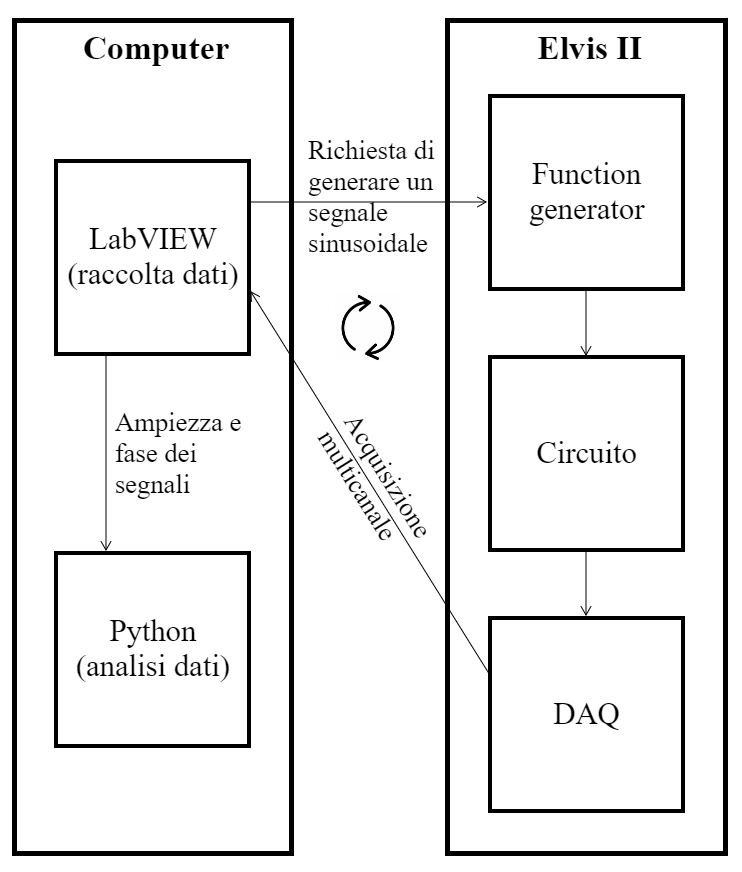
\includegraphics[width=.91\textwidth]{Pipeline_scheme.png}
  \captionof{figure}{\label{fig:schema_pipeline}Schema apparato sperimentale}
\end{minipage}
La componentistica elettrica è stata usata per realizzare il circuito.
È importante notare la bassa resistenza dell'induttanza utilizzata, trascurabile rispetto alle resistenze di carico
(circa $1$ \textOmega), necessaria per la validità di tutte le formule utilizzate in questo articolo.

\subsection{Misure effettuate}
  Abbiamo misurato l'ampiezza del segnale su entrambi i canali in funzione della frequenza, riferita al ground del
  circuito.

  La fase invece è stata misurata rispetto al canale Woofer.
  Si ha quindi che la fase del Tweeter rispetto al Woofer rappresenta in realtà la differenza di fase tra i due riferita
  al generatore, ed è definita come nell'Eq.\,\eqref{eq:p_diff}.


\end{document}